% FONTE TEMA https://github.com/matze/mtheme
%\documentclass[aspectratio=1610]{beamer}
\documentclass[aspectratio=1610, handout]{beamer}
\usepackage[utf8]{inputenc}
\usepackage{ragged2e}
\usepackage{xcolor}
\usepackage[italian]{babel}
\usepackage{multirow}
\usepackage{silence}
\WarningFilter{beamer}{}
\WarningFilter{metropolis}{}
\usetheme[progressbar=frametitle,titleformat=smallcaps]{metropolis}
\setbeamertemplate{frame numbering}[fraction]
\setbeamercovered{dynamic}
\definecolor{rosso}{RGB}{255, 0, 0}
\definecolor{giallo}{RGB}{254,212,23}
\hypersetup{colorlinks=true,linkcolor=black,urlcolor=rosso}
\setbeamercolor{palette primary}{fg=black, bg=giallo}
\setbeamercolor{background canvas}{bg=white}
\setbeamercolor{normal text}{fg=black}
\setbeamercolor{progress bar}{fg=rosso}
\setbeamercolor{framesubtitle}{fg=rosso}
\setbeamercolor{normal text .dimmed}{fg=giallo}
\setbeamercolor{block title alerted}{fg=rosso, bg=giallo}
\setbeamerfont{caption}{size=\tiny}
\setbeamerfont{caption name}{size=\tiny}
\setlength{\abovecaptionskip}{0pt}
\makeatletter
\metroset{block=fill}
\setlength{\metropolis@progressinheadfoot@linewidth}{1pt} 
\setlength{\metropolis@progressonsectionpage@linewidth}{1pt}
\setlength{\metropolis@titleseparator@linewidth}{1pt}
\makeatother

\title{DAL BINARIO AL DECIMALE}
\subtitle{Conversioni tra sistemi di numerazione}
\date{}
\institute{\textit{
        Fonti:
        \begin{itemize}
            \item[-] \href{https://catalogo.sanoma.it/si-op-104157-dal-bit-all-intelligenza-artificiale.html}{Dal BIT all'INTELLIGENZA ARTIFICIALE}
            \item[-] \href{https://it.wikipedia.org/wiki/Sistema_numerico_decimale}{Wikipedia} 
        \end{itemize}
    }
}

\begin{document}

\begin{frame}[plain, noframenumbering]
    \titlepage
\end{frame}

\section{SISTEMA DECIMALE}

\begin{frame}{SISTEMA DECIMALE}
    \begin{alertblock}{DEFINIZIONE}
        \begin{minipage}{0.98\linewidth}
            \justifying
            Per \textbf{sistema numerico decimale} si intende il sistema di \textbf{numerazione posizionale} a 
            base 10 che, per rappresentare i numeri, utilizza dieci cifre da 0 a 9.\\
            \textbf{0 1 2 3 4 5 6 7 8 9}.
        \end{minipage}
    \end{alertblock}
    \pause
    \begin{alertblock}{DEFINIZIONE}
        \begin{minipage}{0.98\linewidth}
            \justifying
            Un \textbf{sistema di numerazione posizionale} è un sistema di numerazione in cui 
            i simboli (cifre), usati per scrivere i numeri, assumono valori diversi a seconda 
            della posizione che occupano nella notazione.
        \end{minipage}
    \end{alertblock}
\end{frame}

\begin{frame}{SISTEMA DECIMALE}
    \only<1 | handout:0>{\begin{figure}
        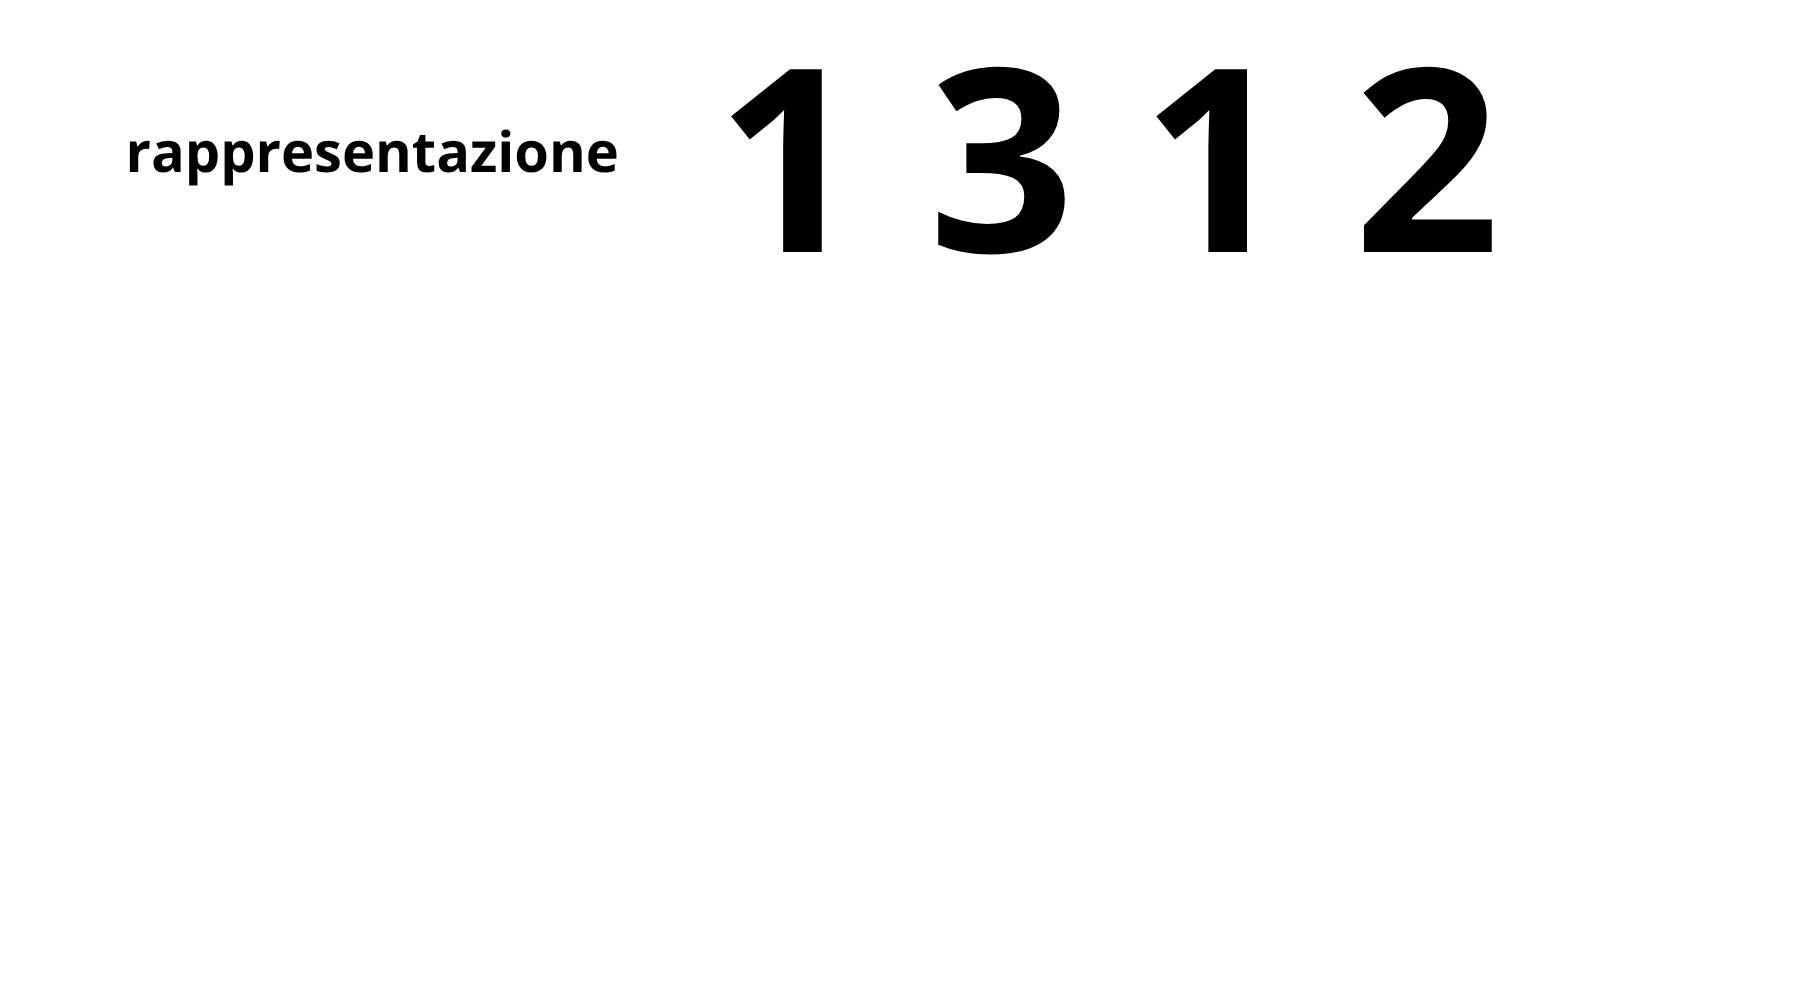
\includegraphics[width=\linewidth]{img/decimale1.png}
        \caption{{creata con \href{www.canva.com}{Canva}}}
    \end{figure}}
    \only<2 | handout:0>{\begin{figure}
        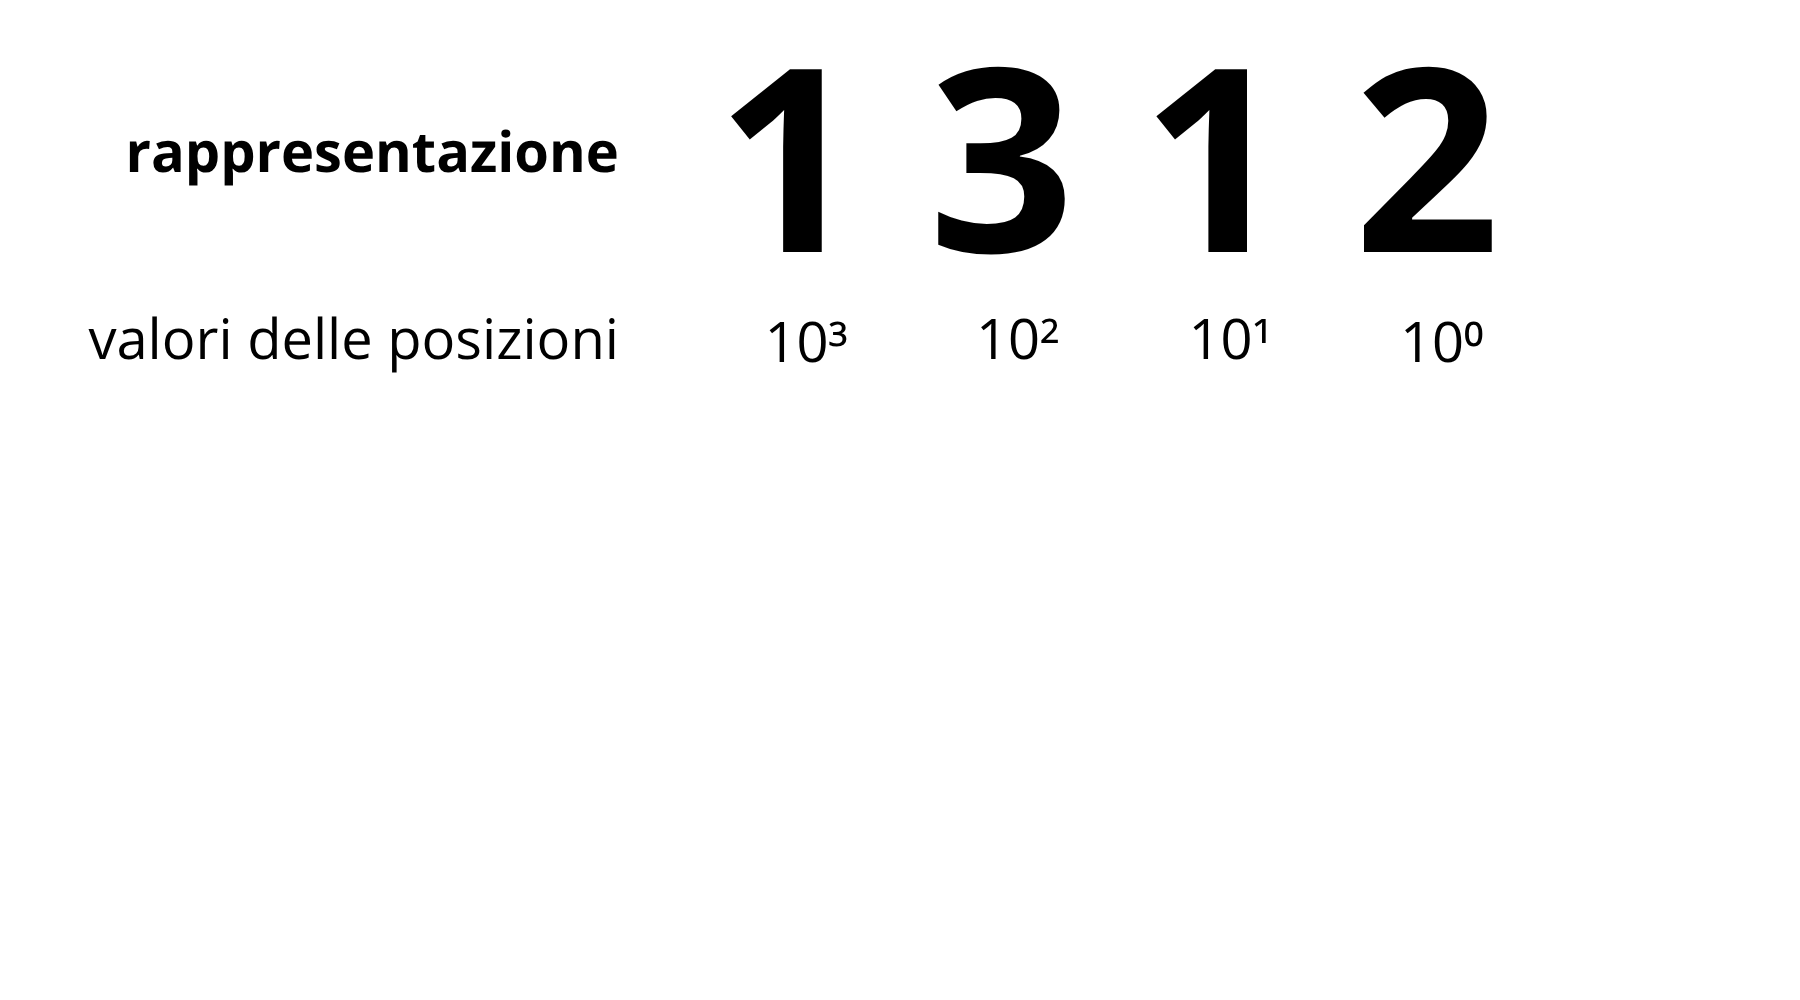
\includegraphics[width=\linewidth]{img/decimale2.png}
        \caption{{creata con \href{www.canva.com}{Canva}}}
    \end{figure}}
    \only<3 | handout:0>{\begin{figure}
        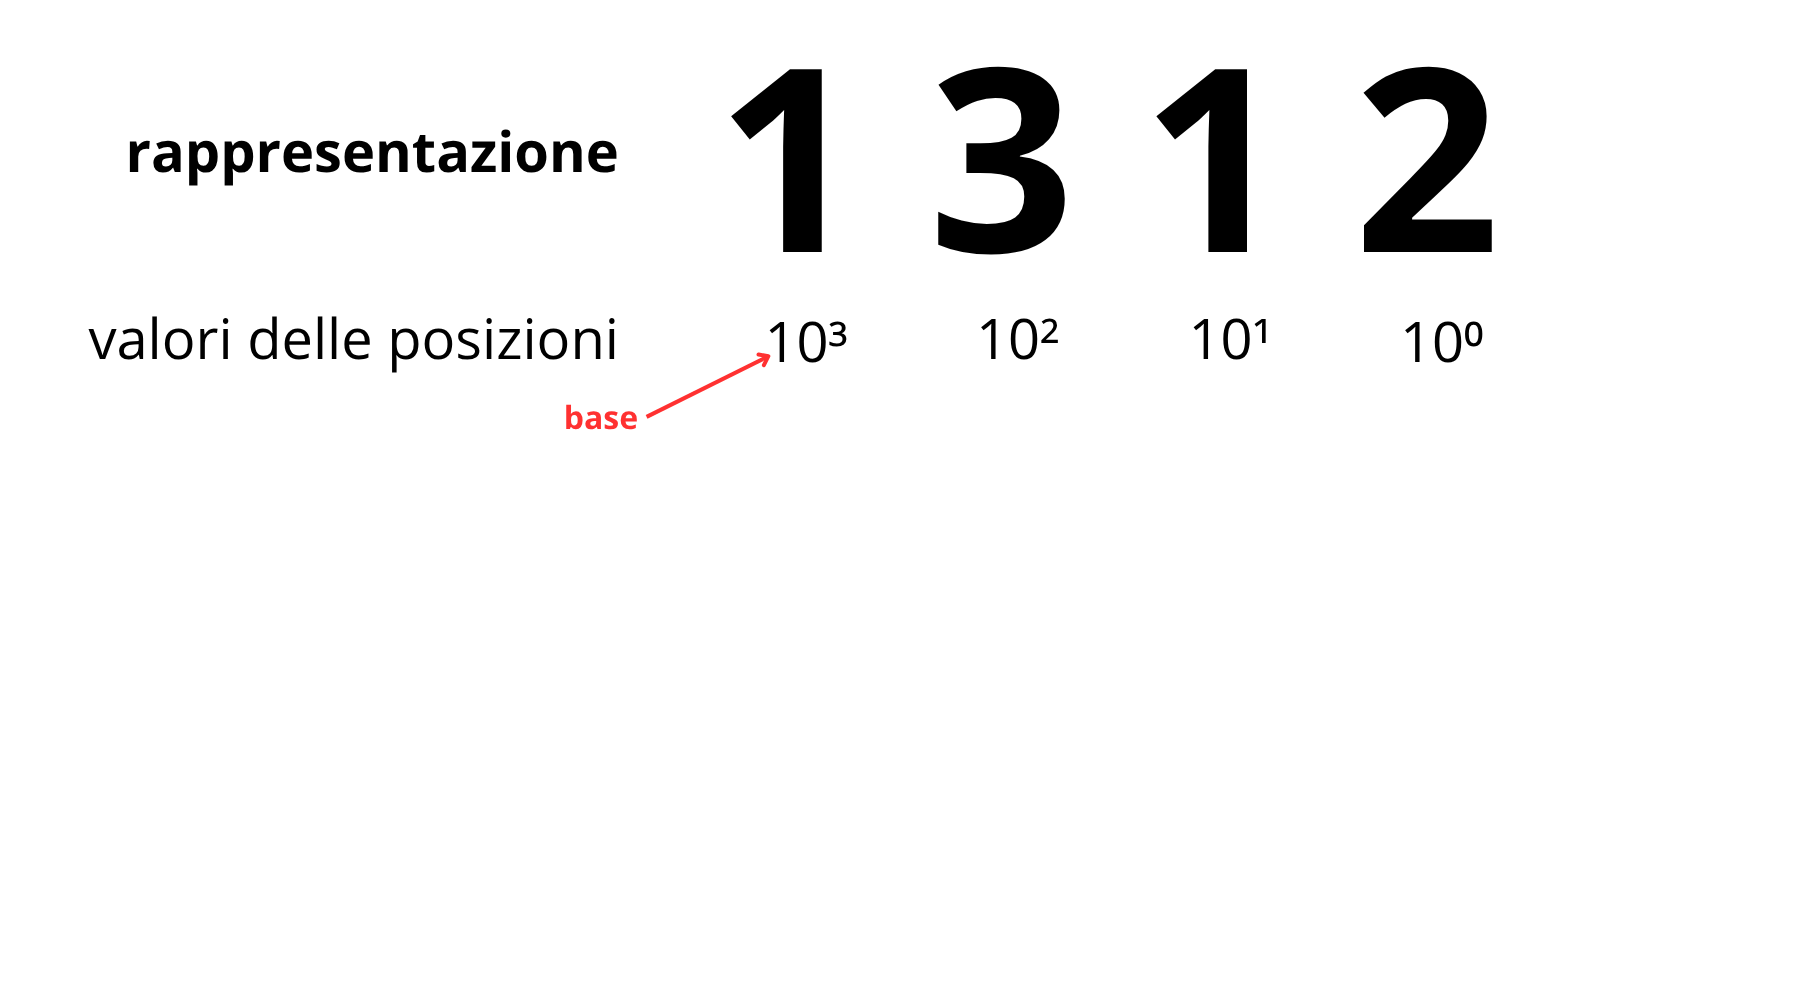
\includegraphics[width=\linewidth]{img/decimale3.png}
        \caption{{creata con \href{www.canva.com}{Canva}}}
    \end{figure}}
    \only<4 | handout:0>{\begin{figure}
        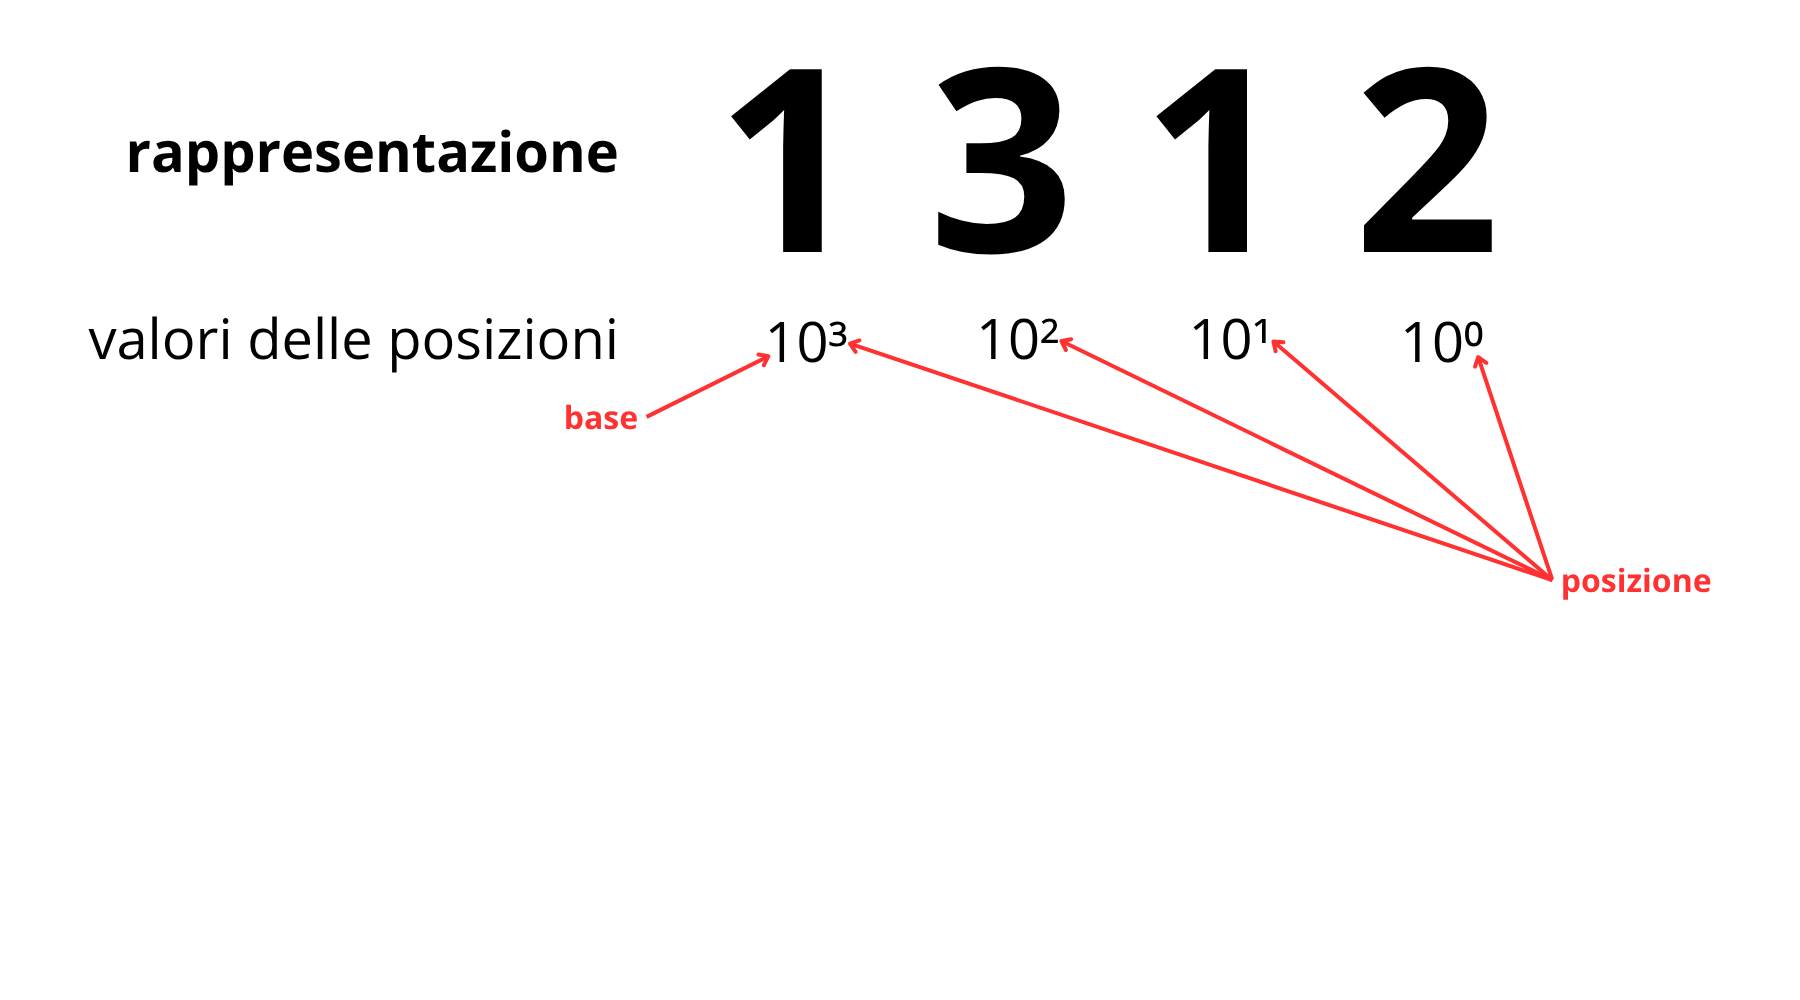
\includegraphics[width=\linewidth]{img/decimale4.png}
        \caption{{creata con \href{www.canva.com}{Canva}}}
    \end{figure}}
    \only<5 | handout:0>{\begin{figure}
        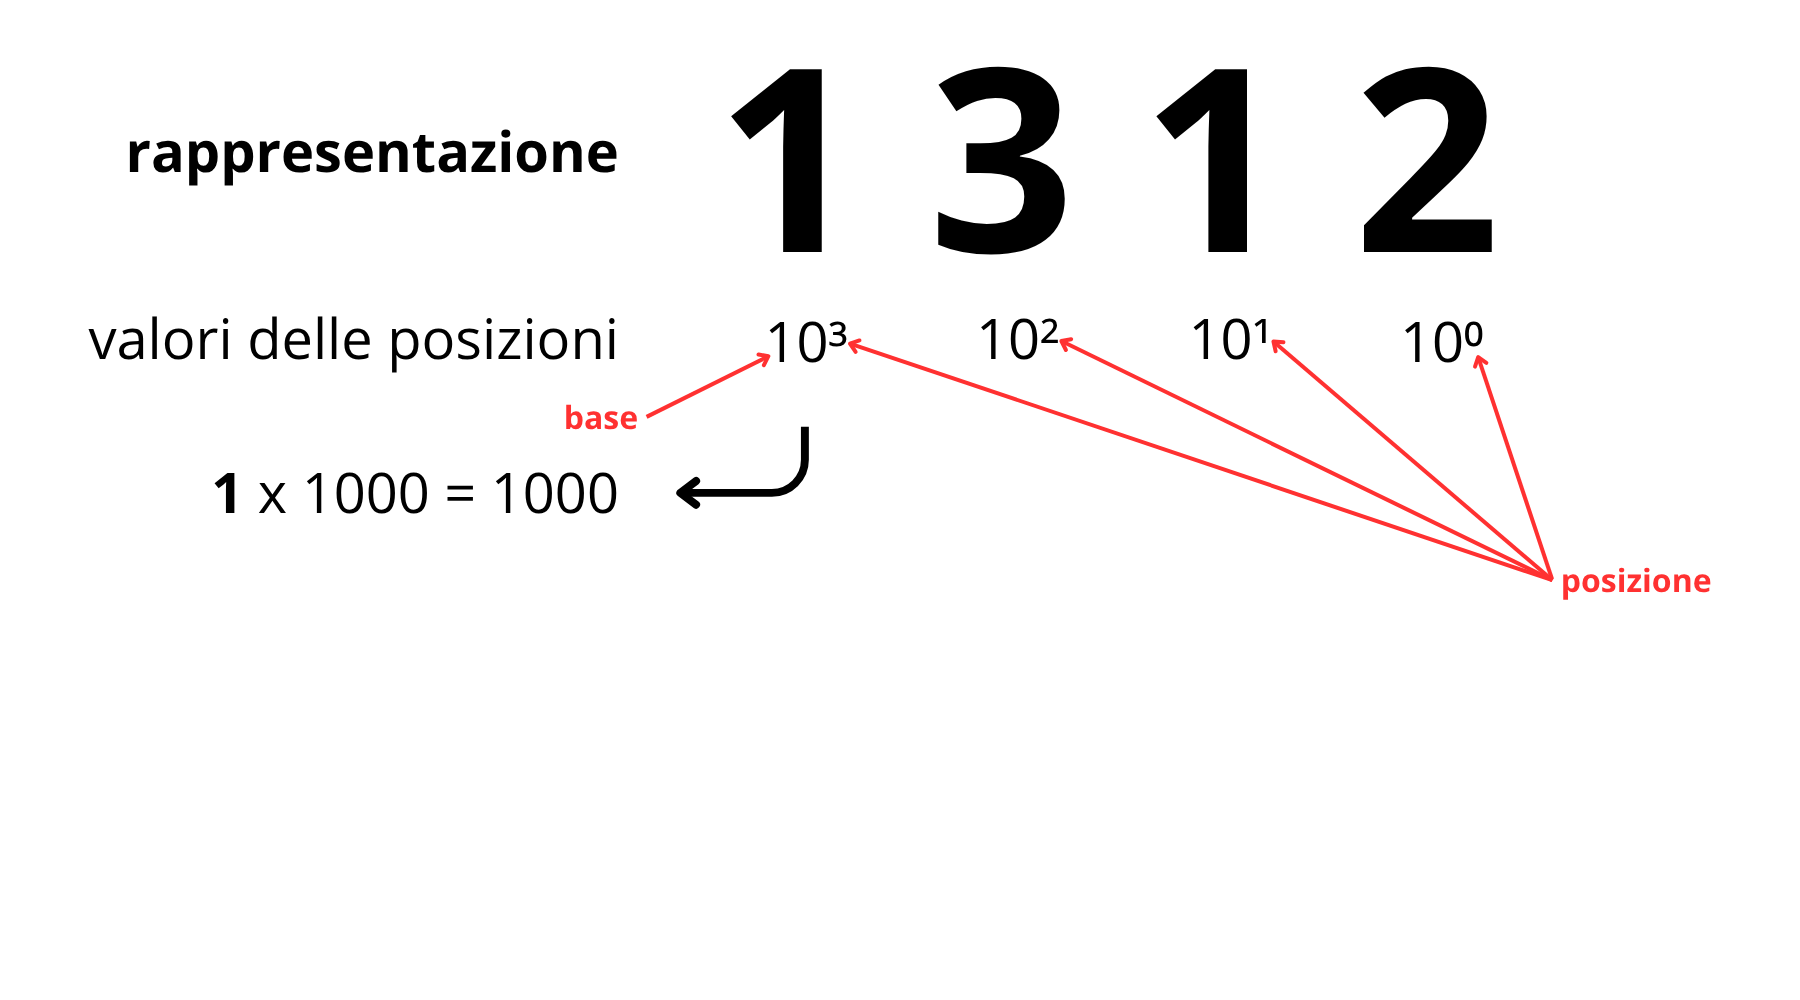
\includegraphics[width=\linewidth]{img/decimale5.png}
        \caption{{creata con \href{www.canva.com}{Canva}}}
    \end{figure}}
    \only<6 | handout:0>{\begin{figure}
        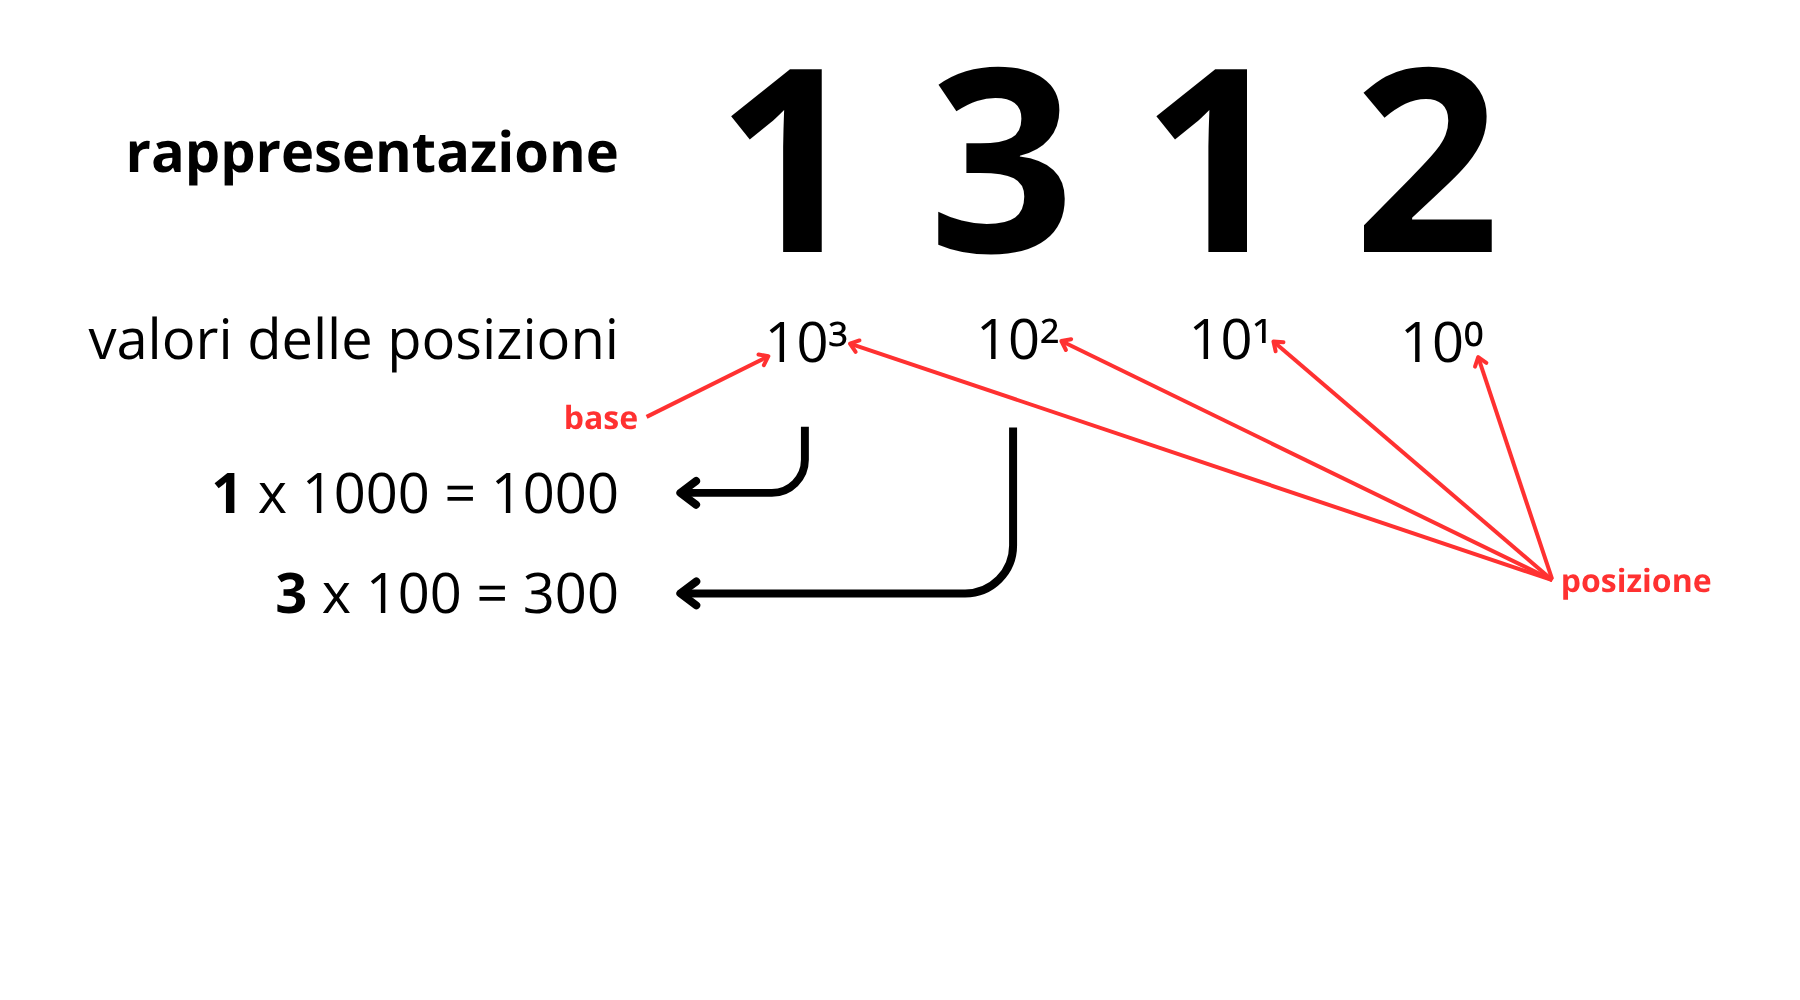
\includegraphics[width=\linewidth]{img/decimale6.png}
        \caption{{creata con \href{www.canva.com}{Canva}}}
    \end{figure}}
    \only<7 | handout:0>{\begin{figure}
        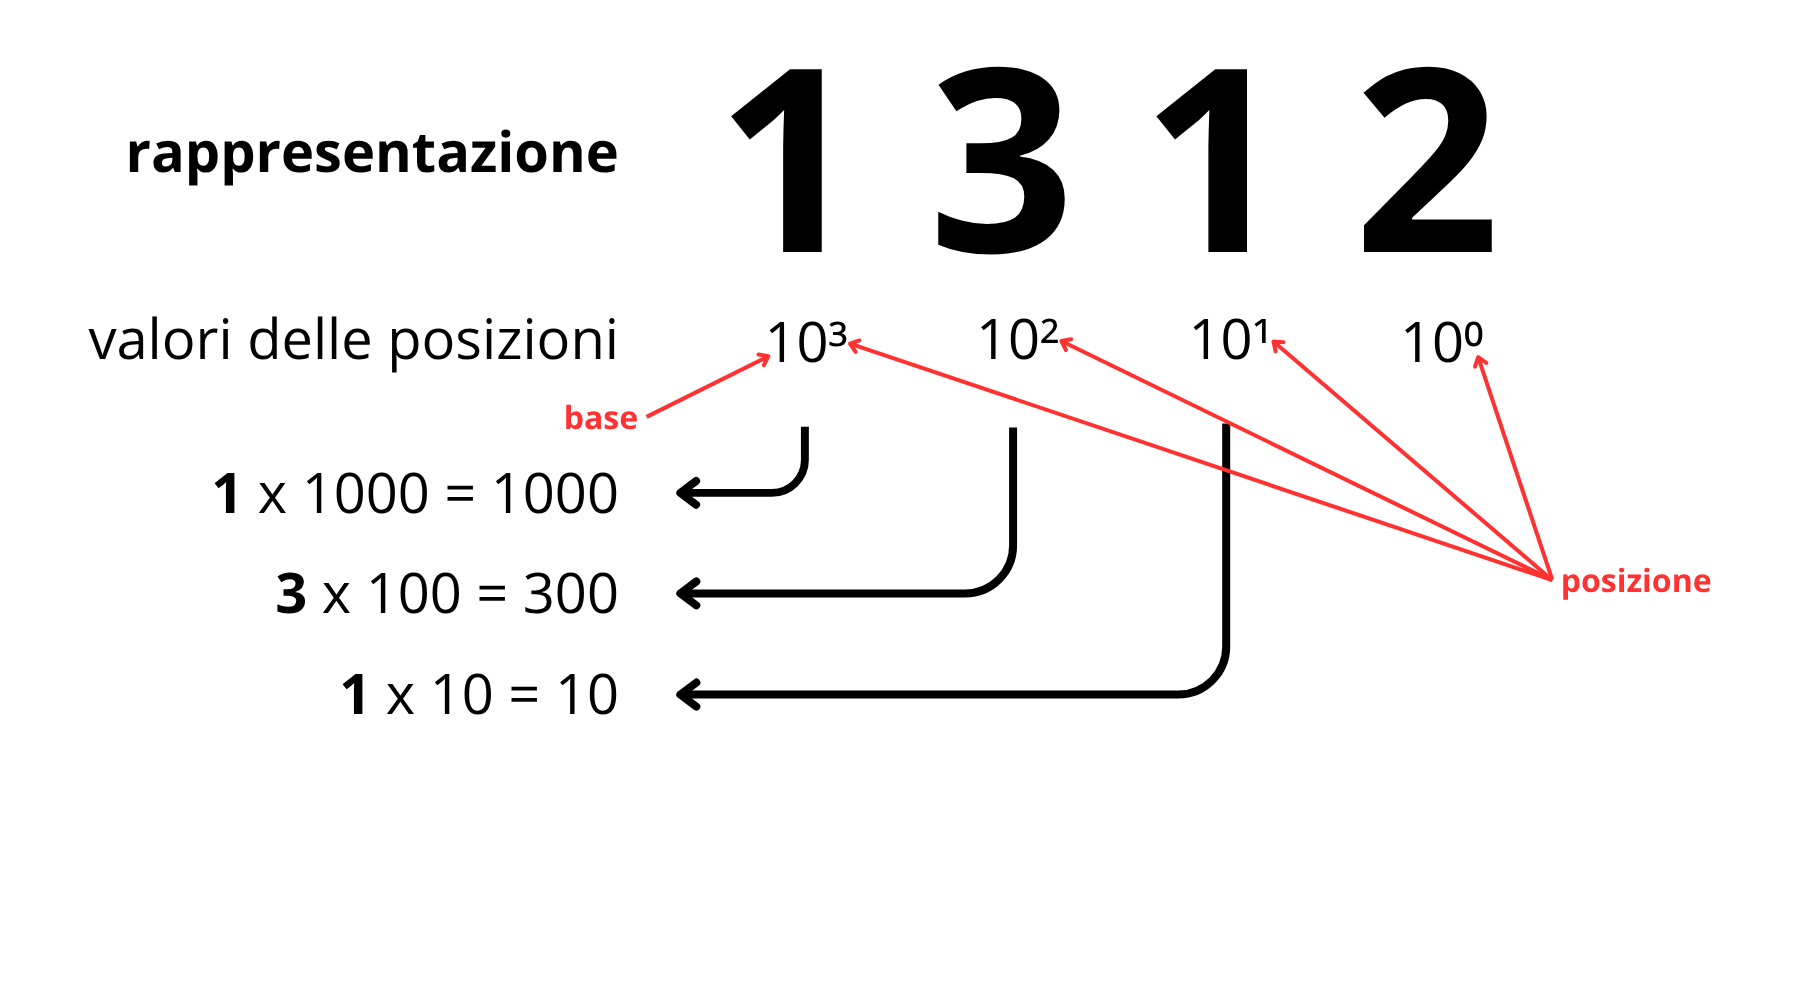
\includegraphics[width=\linewidth]{img/decimale7.png}
        \caption{{creata con \href{www.canva.com}{Canva}}}
    \end{figure}}
    \only<8 | handout:0>{\begin{figure}
        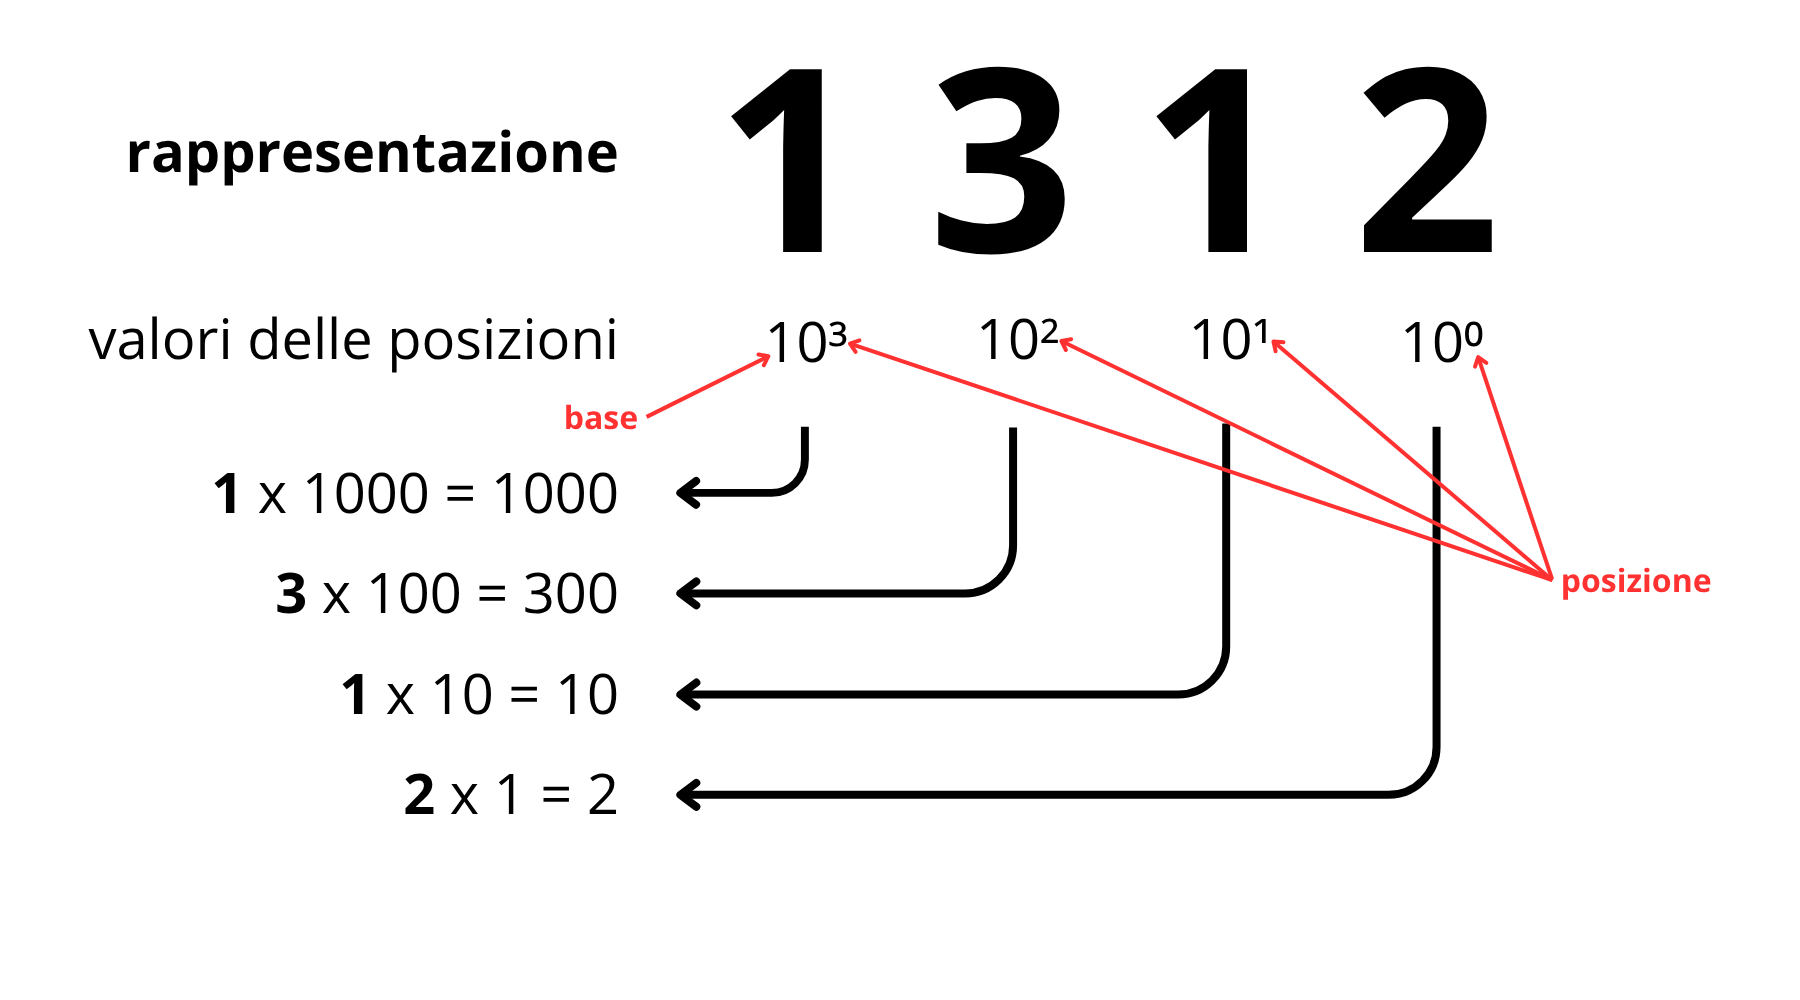
\includegraphics[width=\linewidth]{img/decimale8.png}
        \caption{{creata con \href{www.canva.com}{Canva}}}
    \end{figure}}
    \only<9 | handout:1>{\begin{figure}
        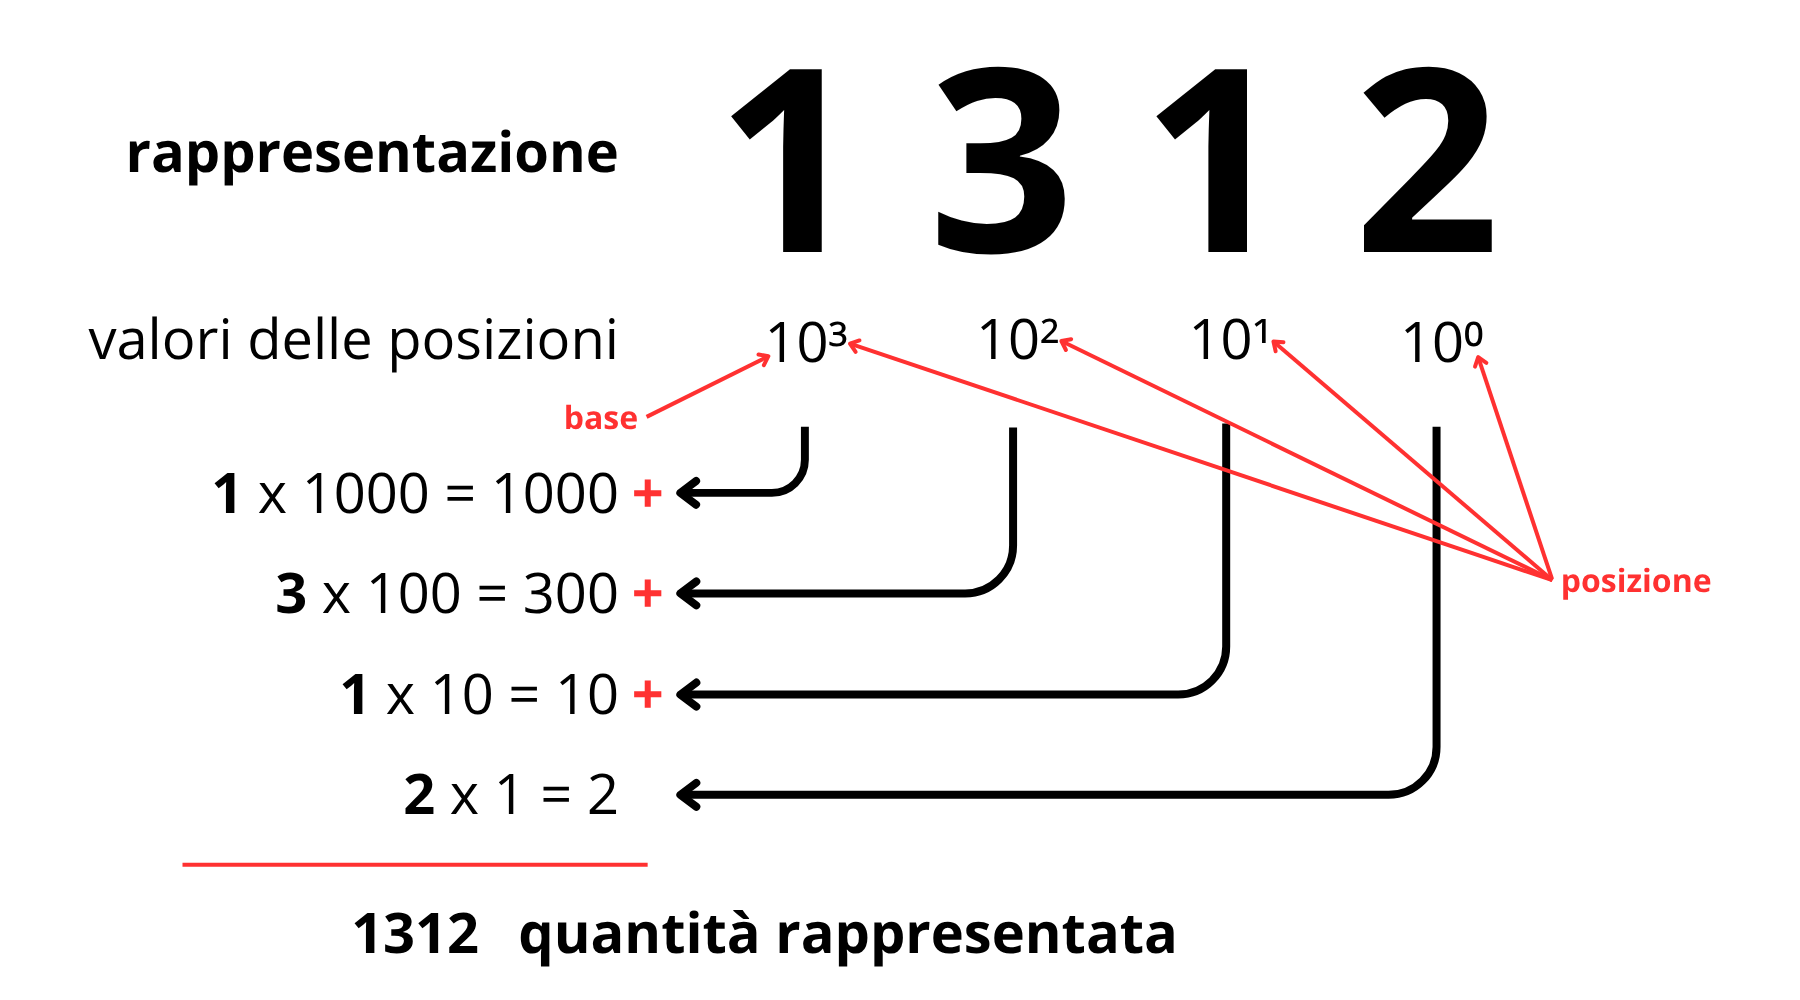
\includegraphics[width=\linewidth]{img/decimale9.png}
        \caption{{creata con \href{www.canva.com}{Canva}}}
    \end{figure}}
\end{frame}

\section{SISTEMA BINARIO}

\begin{frame}{COVERSIONE BINARIO - DECIMALE}
    \centering
    \huge
    \begin{tabular}{c c c c c c c c c c c}
        1 & 0 & 1 & 0 & 0 & 1 & 0 & 0 & 0 & 0 & 0 \\
    \end{tabular}
\end{frame}

\begin{frame}{COVERSIONE BINARIO - DECIMALE}
    \centering
    \begin{tabular}{r||c|c|c|c|c|c|c|c|c|c|c}
        \textbf{NUMERO BINARIO} & \textbf{1} & 0 & \textbf{1} & 0 & 0 & \textbf{1} & 0 & 0 & 0 & 0 & 0 \\
        \hline
        \pause
         & x & x & x & x & x & x & x & x & x & x & x \\
        \hline
         \textbf{PESI} & $\mathbf{2^{10}}$ & $2^9$ & $\mathbf{2^8}$ & $2^7$ & $2^6$ & $\mathbf{2^5}$ & $2^4$ & $2^3$ & $2^2$ & $2^1$ & $2^0$ \\
        \hline
         & = & = & = & = & = & = & = & = & = & = & = \\
        \hline
        \pause
        \textbf{PARZIALI} & \textbf{1024} & 0 & \textbf{256} & 0 & 0 & \textbf{32} & 0 & 0 & 0 & 0 & 0 \\
        \\
        \hline
        \pause
        \textbf{QUANTIT\'A (DECIMALE)} & \multicolumn{11}{c}{$\mathbf{1024 + 256 + 32 = 1312}$} \\
    \end{tabular}
    \pause
    \begin{alertblock}{COVERSIONE BINARIO - DECIMALE}
        \begin{minipage}{0.98\linewidth}
            \centering
            \huge
            $(10100100000)_2 = (1312)_{10}$
        \end{minipage}
    \end{alertblock}
\end{frame}

\end{document}